On pose $e \colon \mathbf{A} \times \mathbf{A} \to \mathbf{G}$ un couplage, où $\mathbf{A}$ est un groupe abélien noté additivement et $\mathbf{G}$ est un groupe abélien noté multiplicativement.
$\mathbf{A}$ et $\mathbf{G}$ sont cycliques de cardinal $p$.

Soit $P$ générateur de $\mathbf{A}$ et $g$ générateur de $\mathbf{G}$ tels que $e(P,P) = g$ (ne marche pas si $e$ est alterné, en particulier pour le couplage de Weil).


\subsection{Diffie-Hellman tripartite}

	Alice choisit $a \in \Z / p\Z$ aléatoire et publie $A = aP \in \mathbf{A}$.
	
	Bob choisit $b \in \Z / p\Z$ aléatoire et publie $B = bP \in \mathbf{A}$.
	
	Carole choisit $c \in \Z / p\Z$ aléatoire et publie $C = cP \in \mathbf{A}$.
	
	Le secret commun est alors
	$$g^{abc} = e(A,B) = e(B,C)^a = e(C,A)^b$$
	Sa sécurité repose sur le problème de DH bilinéaire : retrouver $g^{abc}$ à partir de $A,B,C$.
	
	Variante : DH bilinéaire décisionnel \textrightarrow\ distinguer entre des distributions $(A,B,C,g^{abc})$ et $(A,B,C,g^r)$ avec $r$ aléatoire.
	
	Le couplage est bon pour la crypto si ce problème est réputé dur.


\subsection{Chiffrement basé sur les attributs}

	On va décrire un système à clé publique où :
	\begin{itemize}
		\item[\textbullet] chaque chiffré possède un certain sous-ensemble d'un ensemble possible d'attributs,
		\item[\textbullet] chaque clé de déchiffrement (clé privée d'un utilisateur) possède une politique d'accès,
		\item[\textbullet] une clé déchiffre un message ssi les attributs de ce dernier et la politique d'accès sont compatibles.
	\end{itemize}
	
	\textrightarrow\ protocole KP-ABE (Key Policy - Attribute Based Encryption).
	
	\begin{rem}
		Il existe l'inverse : clé $\leftrightarrow$ attributs et chiffré $\leftrightarrow$ politique, CP-ABE (Ciphertext Policy - ABE).
	\end{rem}
	
	\begin{ex}
		Les chiffrés sont des vidéos avec pour attributs possibles : série, film, comédie, horreur.
		La clé d'Alice permet de déchiffrer les films d'horreur et la clé de Bob permet de déchiffrer des séries ou comédies.
	\end{ex}
	
	Formalisation : soit $U = \{ \bar 1, \ldots, \bar n \}$ l'ensemble des attributs possibles.
	
	La politique est un arbre :
	\begin{itemize}
		\item[\textbullet] feuilles indicées par des éléments de $U$,
		\item[\textbullet] chaque nœud $x$ possède un seul $[k_x]$.
	\end{itemize}
	
	Pour décider si une politique accepte un ensemble d'attributs $V \subset U$, on remonte :
	\begin{itemize}
		\item[\textbullet] une feuille est acceptée si son indice est dans $V$,
		\item[\textbullet] un nœud est accepté si au moins $k_x$ de ses descendants sont acceptés,
		\item[\textbullet] $V$ est compatible à la polique si la racine de l'arbre est acceptée.
	\end{itemize}
	
	\begin{ex}
		$U = \{ \bar 1, \bar 2, \bar 3, \ldots, \bar{10} \}$.
		
		\begin{center}
		\begin{tikzpicture}
		\tikzset{level distance=30pt}
		\Tree [.$[3]$ [.$[1]$ $\bar{1}$ $\bar 3$ $\bar 4$ ]
					  [.$[1]$ $\bar{1}$ $\bar 6$ ] 
					  $\bar 7$ ]
		\end{tikzpicture}
		\end{center}

		%\begin{tikzpicture}[sibling distance=10em,
		  %every node/.style = {shape=rectangle, rounded corners,
			%draw, align=center,
			%top color=white, bottom color=blue!20}]]
		%\node {$[3]$}
			%child { node {$[1]$} }
				%child { node {$\bar 1$} }
				%child { node {$\bar 3$} }
				%child { node {$\bar 4$} }
			%child { node {$[1]$} }
				%child { node {$\bar 1$} }
				%child { node {$\bar 6$} }
			%child { node {$7$} } };
		%\end{tikzpicture}
	\textrightarrow\ déchiffre les messages quui possèdent les attributs (1 ou 3 ou 4) et (1 ou 6) et 7.
	\end{ex}
	
	Le gestionnaire du système possède
	\begin{itemize}
		\item[\textbullet] une clé maîtresse secrète $MK = \{ t_1, \ldots, t_n, y \}$ avev les $t_i \in \Z / p\Z$ et $y \in \Z / p\Z$ aléatoires,
		\item[\textbullet] et une clé publique $PK = \{ T_1, \ldots, T_n, k \}$ où $T_i = t_i P \in \mathbf{A}$ et $k = g^y \in \mathbf{G}$.
	\end{itemize}
	Il peut :
	\begin{enumerate}[1.]
		\item créer des chiffrés avec attributs,
		\item donner aux utilisateurs des clés de déchiffrement avec politique.
	\end{enumerate}
	
	Soit $m \in \mathbf{G}$ un clair à chiffrer avec attributs $V \subset U$.
	
	Le chiffré est $(V, c, \{ E_i \}_{i \in V})$ où $r \in \Z / p\Z$ aléatoire, $c = m k^r \in \mathbf{G}$ et $E_i = r T_i \in \mathbf{A}$.
	
	Clé de déchiffrement associée à un arbre d'accès de haut en bas : pour chaque nœud $x$ on construit un polynôme de degré $\leq k_x - 1$ :
	$$q_x(X) = \lambda_{x,0} + \lambda_{x,1} X + \ldots + \lambda_{x,k_x - 1} X^{k_x - 1}$$
	où $\lambda_{x,1},\ldots,\lambda_{x,k_x - 1}$ sont aléatoires.
	Si $x = x_0$ la racine, $\lambda_{x_0,0} = q_{x_0}(0) = y$.
	Pour les autres nœuds : $\lambda_{x,0} = q_x(0) = q_{\mathrm{parent}(x)}(\mathrm{indice}(x))$ où l'indice de $x$ est $j$ si $x$ est le $j$\up{e} descendant de son parent.
	
	Clé : $D = \{ D_x = t_i^{-1} q_x(0) P \mid x \in \text{feuilles}, i = \mathrm{attribut}(x) \}$.
	
	
	Déchiffrement d'un message d'attributs $V$ du bas vers le haut :
	\begin{itemize}
		\item[\textbullet] $E_i = r T_i = r t_i P$,... TODO
		\item[\textbullet] TODO
	\end{itemize}